\documentclass[conference]{IEEEtran}

\usepackage[T1]{fontenc}
\usepackage[utf8]{inputenc}
\usepackage{times}
\usepackage{amsmath}
\usepackage{graphicx}
\usepackage{float}
\usepackage{booktabs}
\usepackage{array}
\usepackage{xcolor}
\usepackage{tikz}
\usepackage{url}
\usepackage{placeins}
\usepackage[hidelinks]{hyperref}

\usetikzlibrary{arrows.meta,positioning,shapes.geometric}
\graphicspath{{figures/}}
\setcounter{topnumber}{4}
\setcounter{bottomnumber}{2}
\setcounter{totalnumber}{6}
\renewcommand{\topfraction}{0.95}
\renewcommand{\bottomfraction}{0.85}
\renewcommand{\textfraction}{0.08}
\renewcommand{\floatpagefraction}{0.80}

\newcommand{\code}[1]{\texttt{\detokenize{#1}}}
\newcommand{\projecttitle}{AI-Based Food Recognition with Nutrition-Aware Recommendations}
\newcommand{\guide}{Dr. Lavanya Madhuri Bollipo}
\newcommand{\coguide}{Dr. Insha Majeed}

\begin{document}

\title{\projecttitle}

\author{
\IEEEauthorblockN{Jaspreet Singh\IEEEauthorrefmark{1}, Inderpal Singh\IEEEauthorrefmark{2}}
\IEEEauthorblockA{\IEEEauthorrefmark{1}\IEEEauthorrefmark{2}
Department of Computer Science and Engineering\\
National Institute of Technology Srinagar\\
Kashmir 190006, India\\
Email: [student email]
}
\IEEEauthorblockA{Project Guide: \guide\\
Project Co-Guide: \coguide
}
}

\maketitle

\begin{abstract}
This article describes an educational Indian-food recognition application and a reproducibility audit of its evidence. The application joins YOLO11s detection, database nutrition per 100 g, user-estimated gram portions, an explicitly saved browser-only meal journal, and context-labeled recommendations. The existing export contains 48,693 images across 72 classes. A full read-only audit found 138 exact-duplicate groups spanning the original partitions, affecting 276 images, and strict annotation issues in 65 images. Consequently, the previously reported test mAP@50 of 0.820 and mAP@50:95 of 0.680 are historical observations, not estimates of clean independent generalization. Nutrition lookup is available for 19/72 classes with normalized exact matching, 55/72 with automatic matching without precomputed mappings, and 72/72 with the current mapping layer; these counts do not measure nutritional correctness. The work supplies fingerprinted audit artifacts, a source-family-grouped candidate split with quarantine, and an independent mapping-review protocol. It demonstrates an inspectable application and identifies necessary validation work, without claiming a novel detector, measured food mass, or medical efficacy.
\end{abstract}

\begin{IEEEkeywords}
food recognition, nutrition-aware recommendations, YOLO, Indian food dataset, dietary assessment, macronutrients
\end{IEEEkeywords}

\section*{Submission-blocking audit: September 2026}
This is a working draft, not a submission-ready manuscript. A read-only audit of all 48,693 exported images found 138 groups of byte-identical and decoded-pixel-identical images spanning splits (63 train--validation, 56 train--test, and 19 validation--test groups), affecting 276 images. Strict annotation validation also flagged 65 images, including zero-width boxes. Historical detector metrics below are retained for traceability, but do not establish clean held-out generalization. Source exports already include augmented variants, so training-only augmentation in the merged export does not establish independence. Dataset lineage, grouped splitting and independent evaluation must be resolved before submission.

Lookup coverage was 19/72 for normalized exact matching, 55/72 without precomputed mappings and 72/72 for the current mapping layer. These are availability counts, not independently verified correctness. The historical ``VERIFIED'' label is a heuristic macro/mapping check, not clinical or recipe validation. Machine-readable results, fingerprints, review templates and the recovery protocol accompany this repository under \code{research/}.

The September application uses Next.js 16, explicit 25--1,000 g portions in 25 g steps, and browser-only history. Only explicitly saved meals contribute to daily totals. Photos and health selections are not persisted in the journal. Recommendation inputs identify database nutrition per 100 g and do not include selected grams or saved history. Health badges reflect the returned context, not medical certification. Older screenshots depict historical interface states.

A source-family recovery pass then indexed 40,797 source images and joined exact identities with within-export Roboflow filename families. It found 5,548 candidate families spanning old partitions. A deterministic review-only assignment places 26,384 images in train, 5,655 in validation and 5,652 in test, with all 72 classes represented in each. Another 11,002 images are quarantined by whole group for unresolved lineage or annotation review, not deleted. Known group overlap is zero in the candidate partitions, but upstream augmentation, within-group repeats and unrecognized cross-source near duplicates remain limitations. This is preparation for review, not a new benchmark result; the existing detector was not retrained.

\section{Introduction}

Image-based food recognition is often evaluated as a visual classification or detection problem. In a diet-assistance setting, however, the predicted label is only an intermediate result. A class such as \code{palak_paneer}, \code{rice}, or \code{samosa} must be resolved to a nutrition entry before the system can report calories, protein, carbohydrates, or fat. An incorrect resolution can produce a recommendation that appears precise while being nutritionally wrong.

The problem is pronounced in Indian food images. A single meal may contain several dishes, and the same dish may appear under regional names, spelling variants, or dataset-specific labels. Plain rice, for example, may be recorded as \code{WhiteRice}, \code{satham}, or \code{rice}. A chutney label may refer to a side dish or to a small portion attached to a larger item. Visually similar dishes such as biryani and pulao may also differ in ingredient composition and macro values. These cases make direct string matching a weak basis for nutrition lookup.

This paper presents an educational implementation and an evidence audit. YOLO11s predicts visible food labels; the nutrition service selects existing database rows; the frontend scales known per-100-g values by user-estimated grams. Separately, recommendations receive included food names, per-100-g values, a goal and session-only health context. This separation permits software testing but does not demonstrate recipe equivalence or advice quality.

The contributions are:
\begin{enumerate}
    \item a reproducible audit of a 72-class merged export, including exact split overlap, annotation flags and source-family recovery tooling;
    \item a provenance-preserving lookup layer and measured coverage ablation, with independent correctness review still required;
    \item a FastAPI and Next.js prototype that links detection, macro calculation, serving adjustment, and personalized recommendations.
\end{enumerate}

\section{Related Work}

Prior work relevant to this study can be grouped into Indian food recognition, nutrition database alignment, and diet recommendation systems. Methods for depth-based volume estimation and calibrated portion measurement are related, but they are outside the implemented scope because the present system reports database-backed per-100g macro values and leaves serving adjustment to the user.

Indian food recognition studies show that domain-specific data are necessary, but they do not fully address nutrition grounding. IndianFoodNet uses YOLO-style detection for Indian food items and is therefore closer to real meal photographs than single-label classification, where one image is forced into one category \cite{indianfoodnet_2023}. Khana provides a larger Indian cuisine benchmark and reports recurring difficulties such as class imbalance, regional variation, and visual similarity between dishes \cite{khana_dataset_2025}. The Indian Thali study moves toward cluttered meal analysis through segmentation and controlled capture, although such capture assumptions are less convenient for ordinary web uploads \cite{indian_thali_2025}. Lightweight CNN and MobileNetV3 studies support compact architectures and augmentation for food recognition, but their experimental settings remain closer to classification than multi-item detection \cite{lightweight_cnn_food_2022,mobilenetv3_indian_food_2023}. These works motivate a detector trained on Indian food labels, but they leave the detector-to-nutrition link largely under-specified.

Nutrition database work addresses a different part of the problem. The Indian Food Composition Database study shows why cooked Indian foods require dedicated nutrient records rather than direct assumptions from raw ingredients \cite{development_indb_2024}. The Synergistic Frameworks study identifies a practical compatibility gap: visual food labels and food-composition records often differ in spelling, language, or preparation name \cite{synergistic_frameworks_2025}. FKG.in demonstrates how language models and food knowledge graphs can parse regional recipe descriptions, but that setting begins with text rather than an image \cite{fkg_llm_2024}. The present system therefore uses deterministic lookup, reviewed mappings, and recorded source metadata instead of delegating nutrient estimation to a language model.

Recent recommendation systems illustrate both the utility and the risk of generated diet advice. NutriGen and other web-based meal-planning systems generate personalized plans from structured user constraints \cite{nutrigen_2025,genai_meal_planning_2025}. Diet Engine combines food detection with NLP-based dietary guidance and is close to the application direction of this work \cite{diet_engine_2025}. At the same time, evaluations of ChatGPT-style nutrient estimation from meal photographs show that well-formed responses do not guarantee accurate calorie or macro estimates \cite{chatgpt_nutrient_estimation_2025}. The proposed design follows a conservative boundary: recommendations are generated after detection and macro calculation, while the numerical nutrition layer remains database-backed and inspectable.

\section{Proposed System}

Fig.~\ref{fig:pipeline} summarizes the implemented system. The design uses a modular pipeline rather than a single end-to-end predictor because each stage has a different failure mode. Dataset normalization controls the detector label space, YOLO11s performs multi-item food detection, the nutrition layer resolves labels to database rows, and the recommendation module receives structured macro values. YOLO11s was selected as a compact detector suitable for a web prototype where inference time, model size, and multi-object localization are practical constraints. Recommendation text is generated only after the backend has calculated nutrition values.

\begin{figure}[!tbp]
\centering
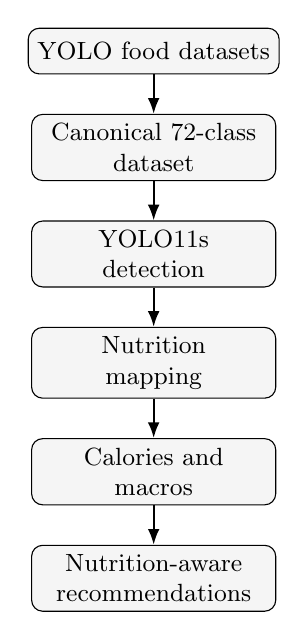
\begin{tikzpicture}[
    node distance=0.50cm,
    block/.style={draw, rounded corners, align=center, minimum width=3.10cm, minimum height=0.58cm, fill=gray!8, font=\small},
    arrow/.style={-{Latex[length=2mm]}, thick}
]
\node[block] (data) {YOLO food datasets};
\node[block, below=of data] (canon) {Canonical 72-class\\dataset};
\node[block, below=of canon] (model) {YOLO11s\\detection};
\node[block, below=of model] (mapping) {Nutrition\\mapping};
\node[block, below=of mapping] (macros) {Calories and\\macros};
\node[block, below=of macros] (rec) {Nutrition-aware\\recommendations};
\draw[arrow] (data) -- (canon);
\draw[arrow] (canon) -- (model);
\draw[arrow] (model) -- (mapping);
\draw[arrow] (mapping) -- (macros);
\draw[arrow] (macros) -- (rec);
\end{tikzpicture}
\caption{End-to-end workflow for AI-based food recognition with nutrition-aware recommendations.}
\label{fig:pipeline}
\end{figure}

Let a detector return
\begin{equation}
D_x=\{(\hat{c}_q,b_q,p_q)\}_{q=1}^{Q_x},
\end{equation}
where $\hat{c}_q$ is the predicted food class, $b_q$ is the bounding box, and $p_q$ is the confidence score. Let the nutrition database be
\begin{equation}
N=\{(n_j,\mathbf{m}_j,z_j)\}_{j=1}^{L},
\end{equation}
where $n_j$ is a food name, $\mathbf{m}_j=[e_j, protein_j, carb_j, fat_j]$ is the nutrition vector, and $z_j$ stores source metadata.

The following rule summarizes offline mapping construction. Runtime first uses precomputed entries, then normalized exact matching, containment with a length ratio of at least 0.5, variation containment, and last-resort fuzzy matching at 0.4. The offline 0.78 threshold does not govern every runtime fallback. These rules are preserved, not certified as clinically appropriate:
\begin{equation}
\resizebox{0.98\columnwidth}{!}{$
M(c)=
\begin{cases}
M_{\mathrm{manual}}(c), & \text{if a precomputed mapping exists},\\
M_{\mathrm{exact}}(c), & \text{if normalized names match},\\
M_{\mathrm{sup}}(c), & \text{if an accepted supplemental row exists},\\
M_{\mathrm{fuzzy}}(c), & \text{if score}(c,n)\geq0.78,\\
\emptyset, & \text{otherwise}.
\end{cases}
$}
\label{eq:mapping}
\end{equation}
The last case is a deliberate design choice. If no accepted nutrition match exists, the system keeps the detection visible but does not assign macro values. For a diet-assistance interface, an explicit missing value is preferable to a confident but unsupported nutrient estimate.

For a meal image, the displayed macro vector is
\begin{equation}
\hat{\mathbf{m}}_{\mathrm{known}}(x)=\sum_{q:M(\hat{c}_q)\ne\emptyset}s_q\mathbf{m}_{M(\hat{c}_q)},
\end{equation}
Here $s_q=w_q/100$ for an included detection with user-estimated weight $w_q$ in grams, and $s_q=0$ for an excluded detection. Unknown nutrition is omitted from the known subtotal and separately marks the estimate incomplete, not zero. Portions default to 100 g and range from 25 to 1,000 g in 25 g steps. The image does not measure food mass. Only saved meals contribute to local-day totals; a successful scan alone records no consumption.

\subsection{Runtime Data Contract}

The backend response is structured so that the frontend does not infer missing or approximate values from presentation logic. Each detection carries the raw detector label, display name, confidence score, bounding box, image dimensions, macro values, nutrition unit, nutrition source, and missing-nutrition flag. If no valid food is detected, the API returns an explicit no-food state. If a detected class has no accepted nutrition match, the detection remains visible while macro values remain unavailable. The interface exposes source metadata and approximate mapping notes. Successful lookup does not establish equivalence with the photographed dish.

\section{Dataset Construction}

Five source exports were merged into one label-normalized dataset \cite{source_project_z0tql,source_microplastics,source_indianfood7,source_indianfoodnet,source_south_indian}. Their names and class orders differ, so source labels were normalized for case, punctuation and selected semantic aliases before rewriting YOLO class indices. This engineering step preserves multi-food annotation rows but does not establish independent source families or resolve image-level reuse rights. The September audit qualifies all downstream detector claims.

\begin{table}[!tbp]
\centering
\caption{Source dataset pool before project-specific merging.}
\label{tab:source-datasets}
\scriptsize
\begin{tabular}{>{\raggedright\arraybackslash}p{0.43\linewidth}rrrr}
\toprule
Source dataset & Classes & Train & Valid & Test\\
\midrule
Indian food detection v1 & 17 & 7547 & 1053 & 453\\
Indian food v6 & 29 & 8088 & 213 & 105\\
Indian food v2 subset & 7 & 1698 & 159 & 92\\
IndianFoodNet YOLO export & 30 & 11387 & 1073 & 576\\
South Indian food detection v19 & 31 & 6478 & 1294 & 581\\
\bottomrule
\end{tabular}
\end{table}

\begin{table}[!tbp]
\centering
\caption{Representative groups in the 72-class Indian-food label space.}
\label{tab:class-groups}
\scriptsize
\begin{tabular}{>{\raggedright\arraybackslash}p{0.25\linewidth}>{\raggedright\arraybackslash}p{0.58\linewidth}}
\toprule
Group & Example classes\\
\midrule
Rice dishes & \code{rice}, \code{lemon_rice}, \code{sambar_satham}, \code{veg_briyani}\\
Breads & \code{roti}, \code{paratha}, \code{bhakri}, \code{bhatura}, \code{puri}\\
Curries & \code{chole}, \code{rajma_curry}, \code{fish_curry}, \code{palak_paneer}\\
Snacks & \code{samosa}, \code{onion_pakoda}, \code{medu_vada}, \code{khandvi}\\
Sweets & \code{gulab_jamun}, \code{ras_malai}, \code{kheer}, \code{jalebi}\\
Sides & \code{coconut_chutney}, \code{green_chutney}, \code{raita}, \code{salad}\\
\bottomrule
\end{tabular}
\end{table}

\begin{table}[!tbp]
\centering
\caption{Generated dataset split summary.}
\label{tab:dataset}
\begin{tabular}{lr}
\toprule
Item & Result\\
\midrule
Canonical food classes & 72\\
Train image-label pairs & 36,852\\
Validation image-label pairs & 5,922\\
Archived test image-label pairs & 5,919\\
Total exported pairs & 48,693\\
Classes with visual samples & 72 / 72\\
Strict-audit flagged images & 65\\
\bottomrule
\end{tabular}
\end{table}

The generated dataset used a 70/15/15 target ratio. Multi-label images were retained. Additional augmentation was restricted to training, but some source exports already contained augmented variants. The September audit found identical images spanning partitions; independence cannot be inferred from this splitting procedure.

A visual verification script sampled real images for every class and generated contact sheets. This check confirmed that all 72 classes had image samples after merging. It also found three local annotation issues: one \code{jalebi} sample that did not visually match jalebi, one \code{kaara_chutney} box placed on a vada, and one extremely thin \code{nandu_masala} box. These issues were retained as documented dataset defects rather than treated as class-order errors.

\begin{figure}[!tbp]
\centering

\includegraphics[width=\linewidth,height=0.22\textheight,keepaspectratio]{class_verification_page_01.jpg}
\caption{Sample visual verification sheet generated from real exported dataset images.}
\label{fig:class-verification}
\end{figure}

\FloatBarrier

\section{Historical Detector Training and Evaluation}
\suppressfloats[t]

The final detector was trained with YOLO11s using 640-pixel images and batch size 16. Training resumed from epoch 56 and continued to epoch 100 on a Tesla T4 GPU. This configuration was chosen to keep the detector small enough for prototype inference while retaining multi-object localization, which is required for meal images containing more than one food item. The best logged validation mAP@50 was 0.83379 at epoch 78. On the archived test split, the exported model reached 0.842 precision, 0.801 recall, 0.820 mAP@50, and 0.680 mAP@50:95 across 5,919 images and 8,875 instances.

\begin{table}[H]
\centering
\caption{Historical detector metrics on overlapping partitions; not an independent benchmark.}
\label{tab:detector-metrics}
\begin{tabular}{lrrrr}
\toprule
Split & Precision & Recall & mAP@50 & mAP@50:95\\
\midrule
Validation & 0.847 & 0.807 & 0.830 & 0.692\\
Archived test & 0.842 & 0.801 & 0.820 & 0.680\\
\bottomrule
\end{tabular}
\end{table}

\begin{figure}[H]
\centering
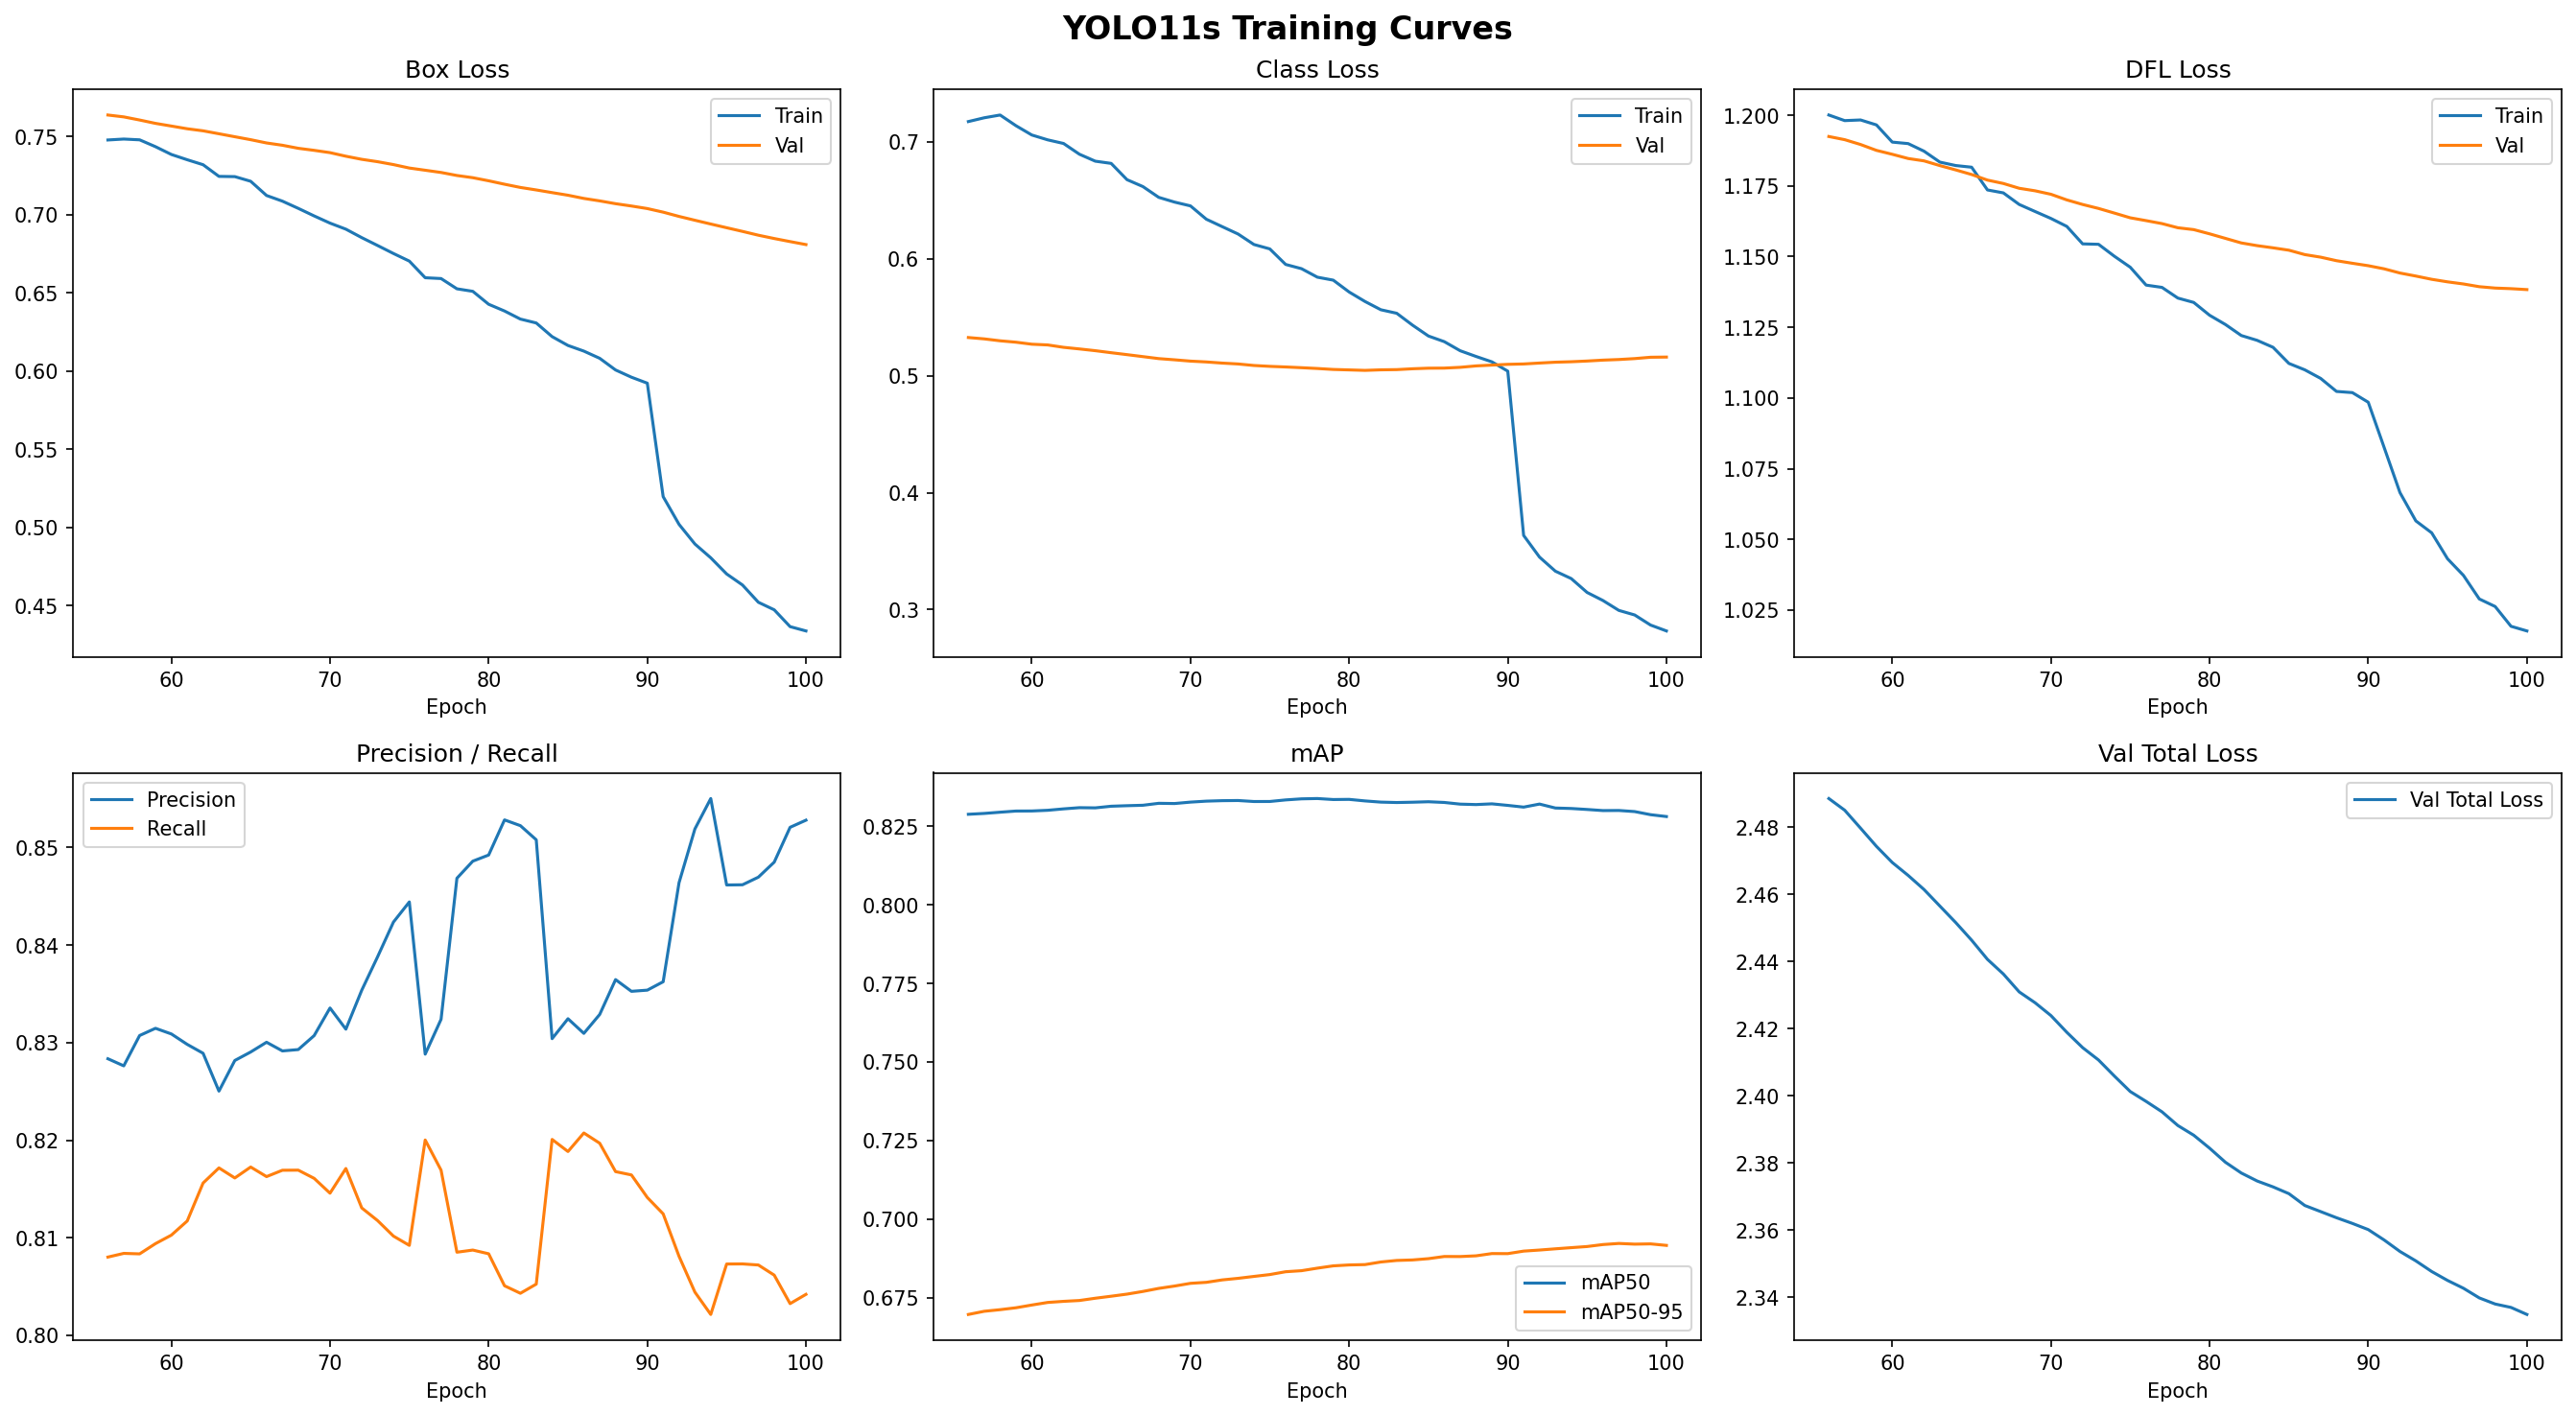
\includegraphics[width=\linewidth,height=0.23\textheight,keepaspectratio]{yolo11s_training_curves.png}
\caption{YOLO11s training curves for the 72-class Indian-food detector.}
\label{fig:training-curves}
\end{figure}

\begin{figure}[H]
\centering
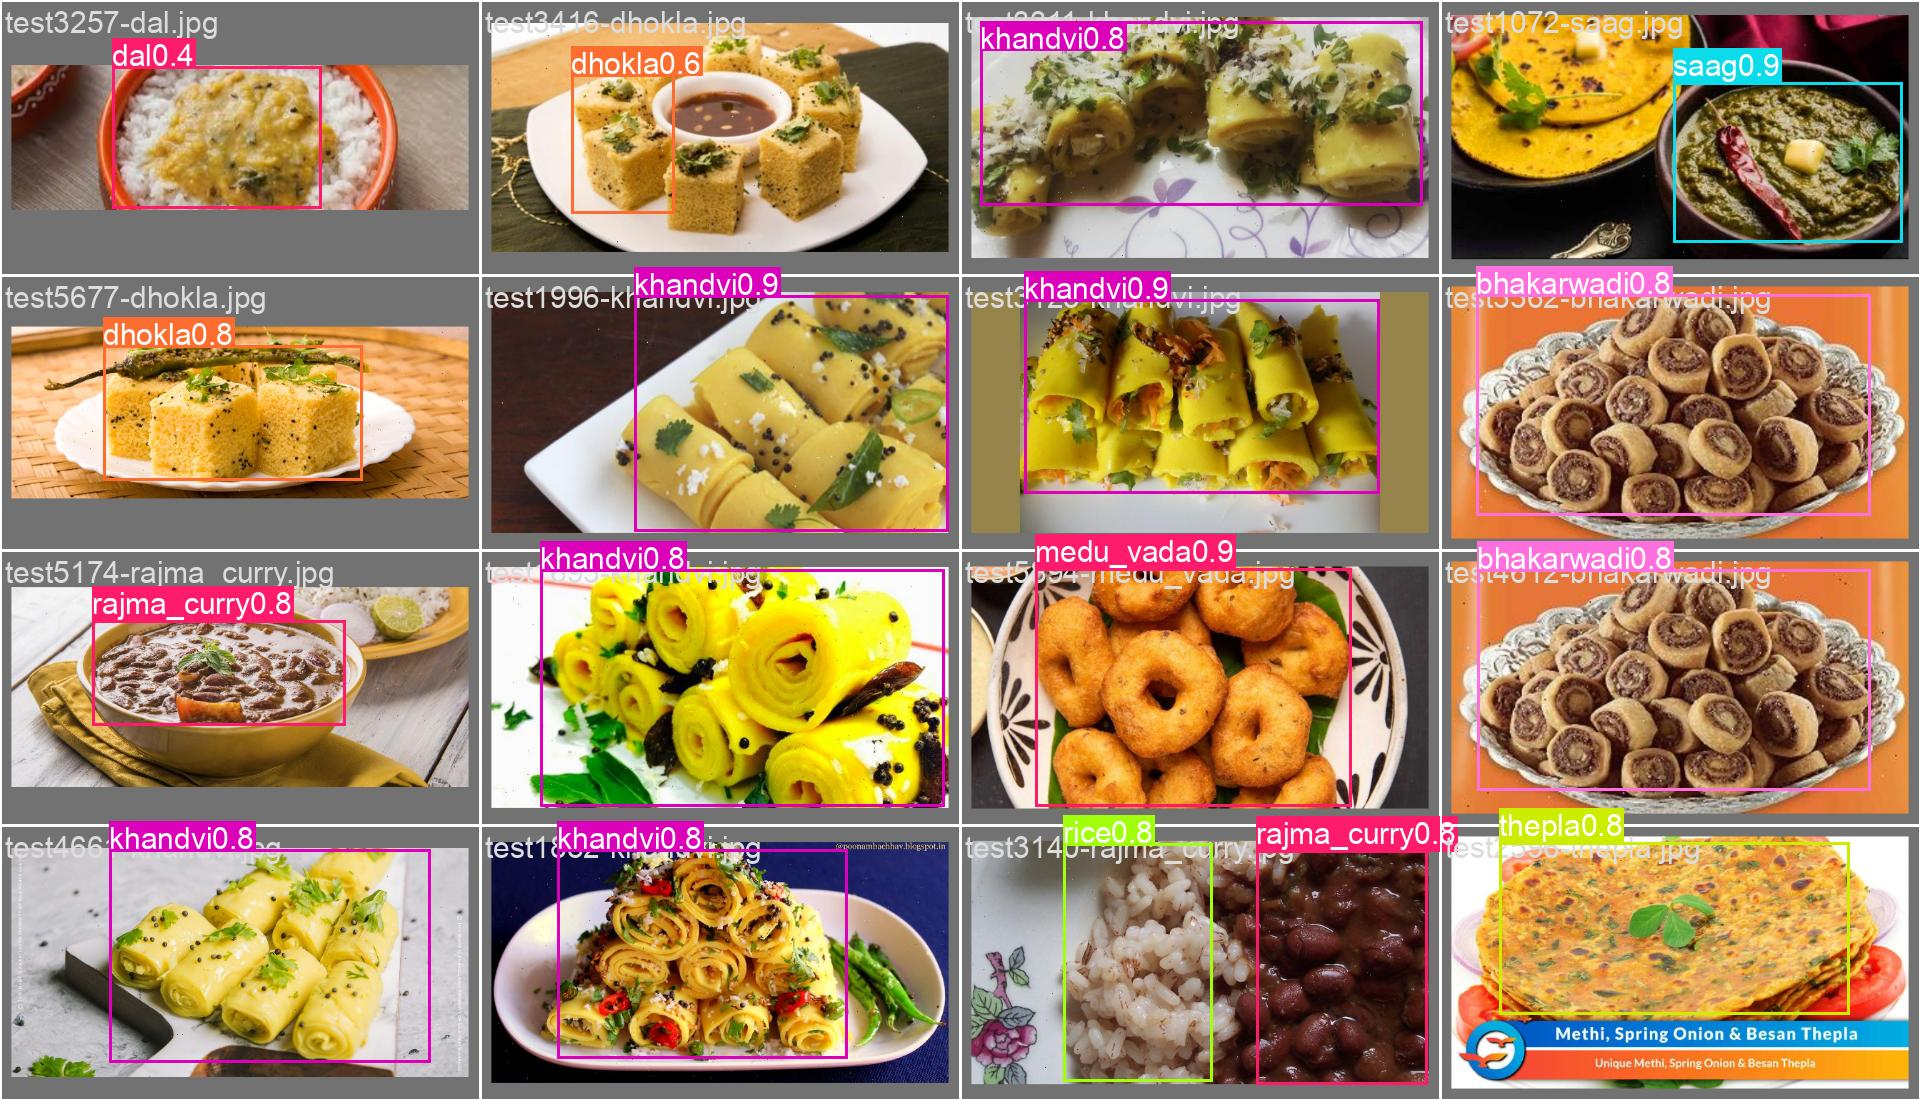
\includegraphics[width=\linewidth,height=0.22\textheight,keepaspectratio]{yolo11s_test_predictions.jpg}
\caption{Example archived test predictions from the final YOLO11s detector.}
\label{fig:test-predictions}
\end{figure}

The archived validation and test metrics are numerically close, but this does not rule out leakage. The confirmed split overlap prevents treating these numbers as proof of independent generalization. Confusion matrices and qualitative predictions remain descriptive historical artifacts; source-grouped evaluation and per-class analysis are required before stronger claims.

\begin{figure}[!tbp]
\centering
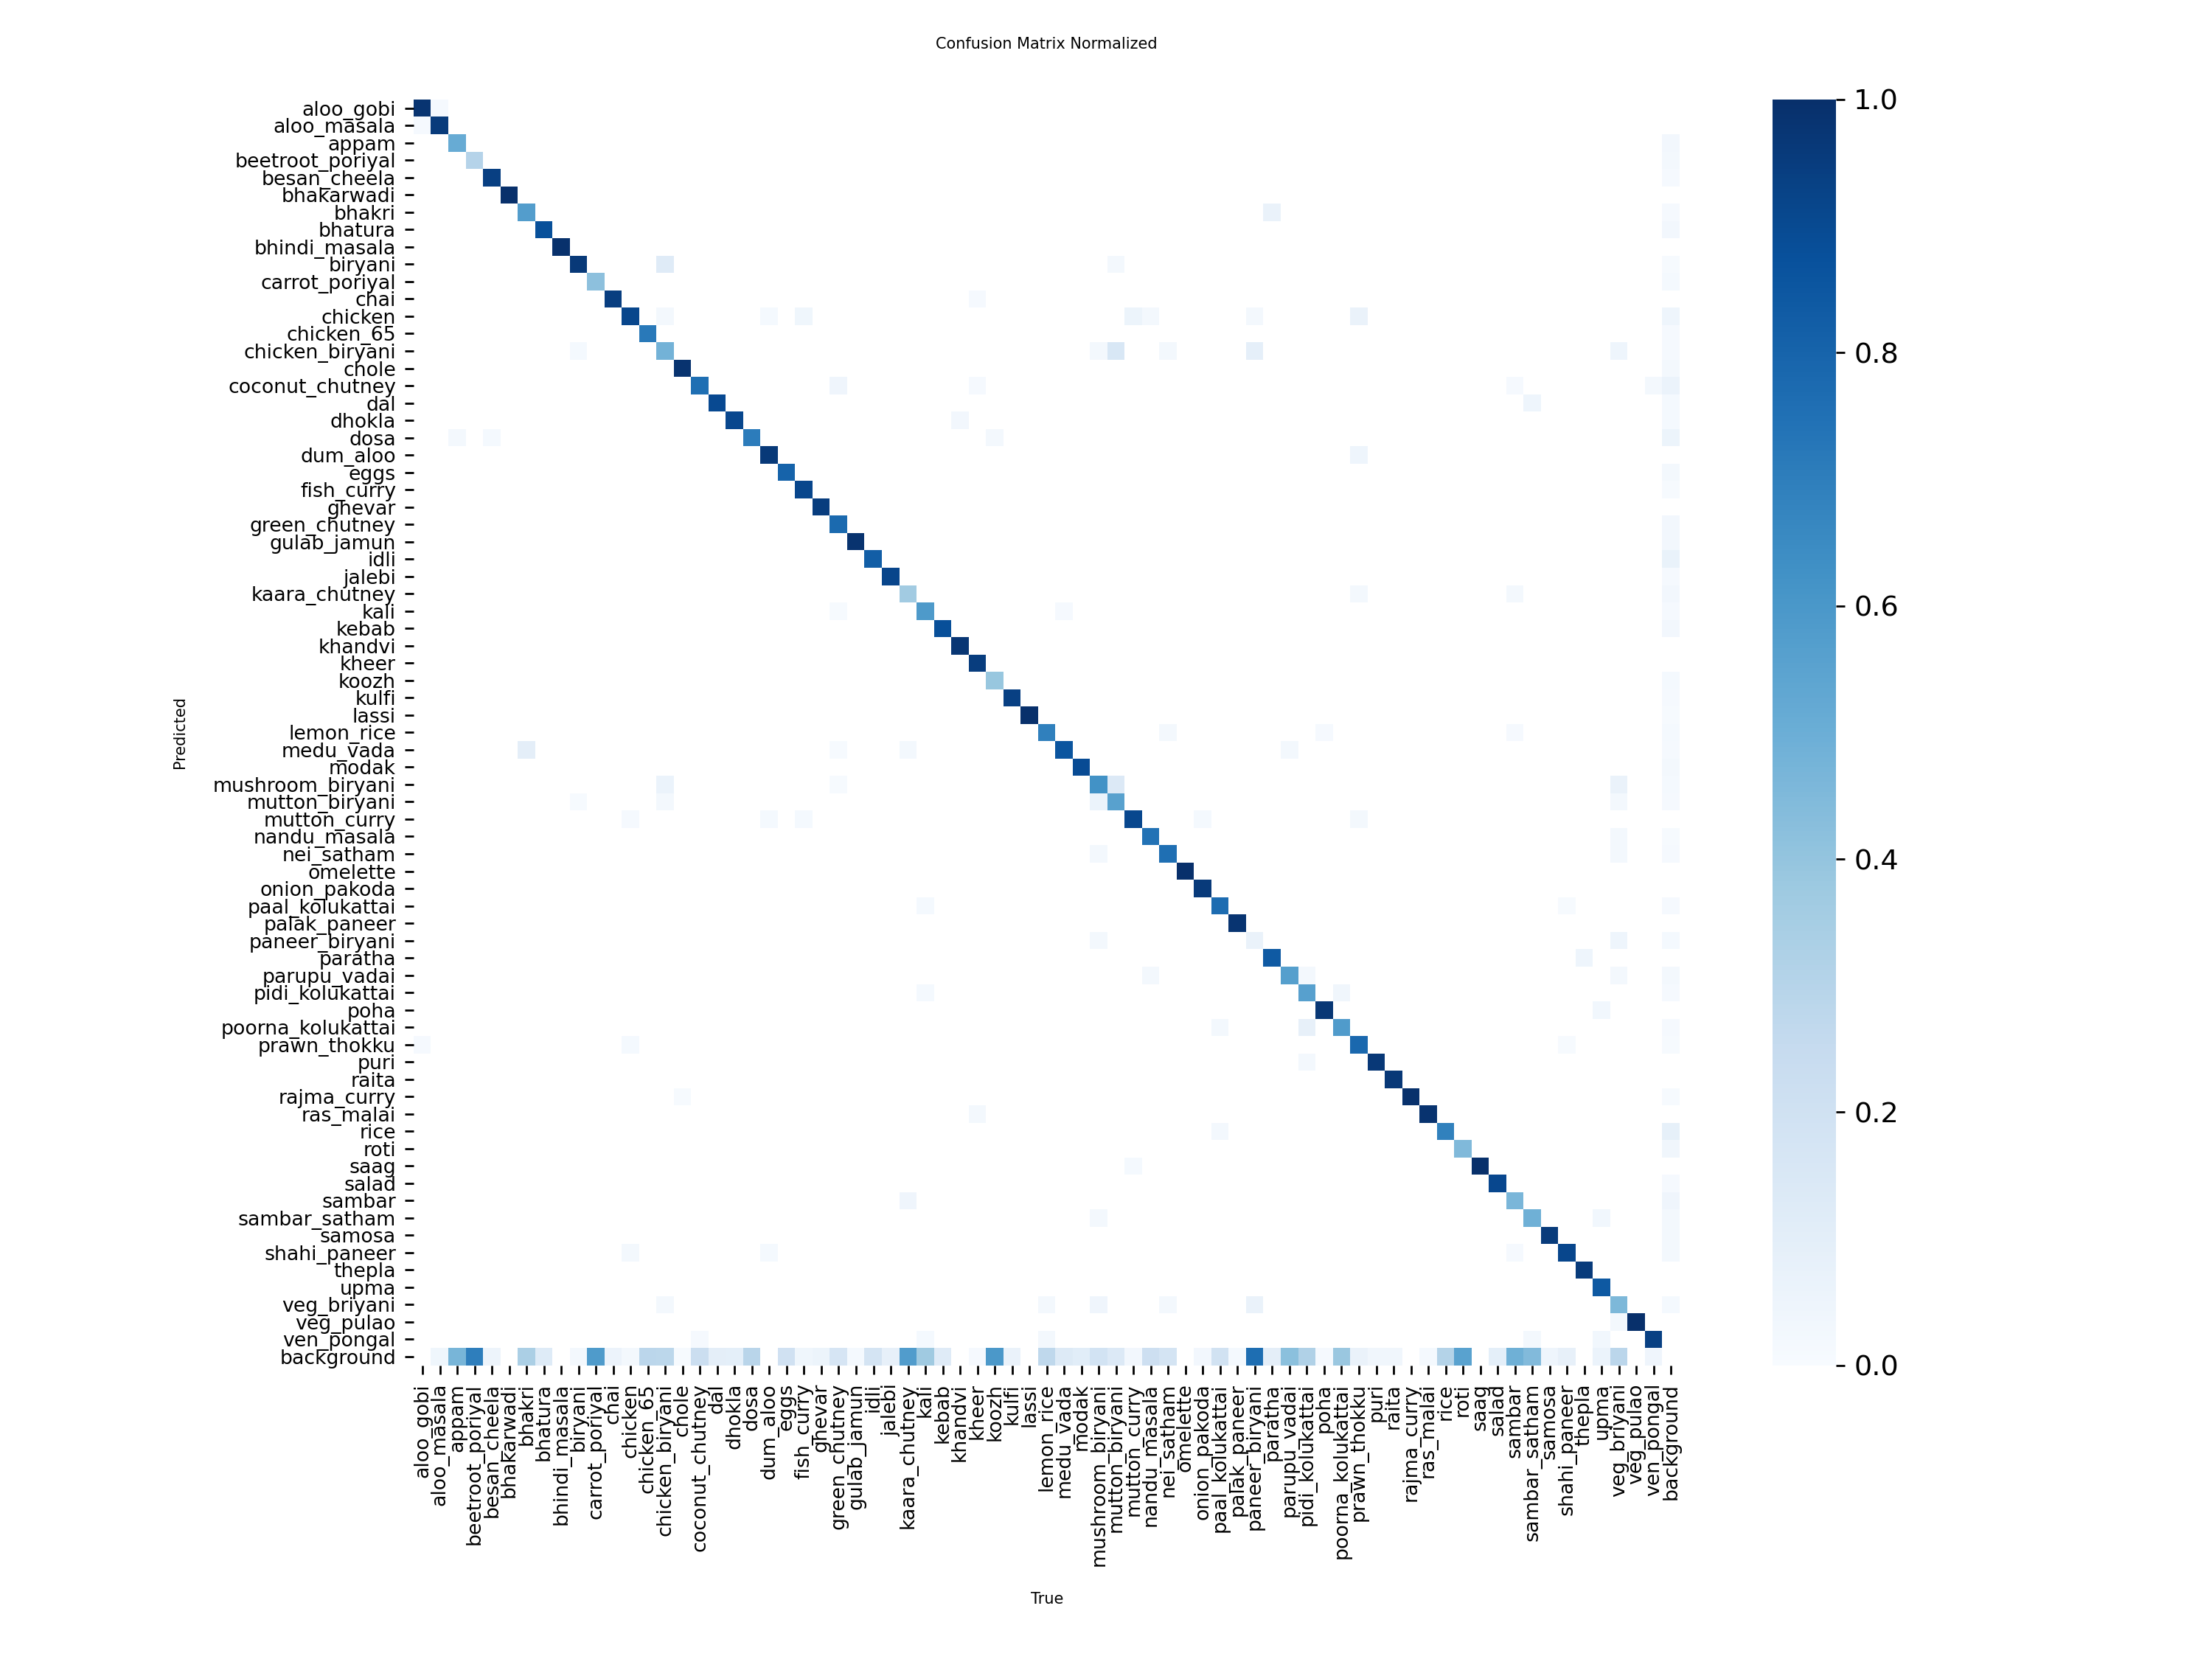
\includegraphics[width=\linewidth,height=0.23\textheight,keepaspectratio]{yolo11s_test_confusion_matrix_normalized.png}
\caption{Normalized confusion matrix from archived test evaluation.}
\label{fig:confusion-matrix}
\end{figure}

\FloatBarrier

\section{Nutrition Mapping and Recommendations}
\suppressfloats[t]

The SQLite database imports the \textit{Indian Nutrient Databank} workbook from the authors' public repository \cite{development_indb_2024,indb_artifact_2024}. The local workbook is byte-identical to the pinned upstream artifact; its fingerprint and source revision are recorded in \code{research/evidence/nutrition-provenance.json}. Artifact identity does not establish permissions for every upstream input or validate nutrient values independently. The table contains 1,010 rows, including five supplements for \code{bhakarwadi}, \code{ghevar}, \code{jalebi}, \code{khandvi}, and \code{nandu_masala} \cite{fatsecret_bhakarwadi_2026,clearcals_ghevar_2026,clearcals_jalebi_2026,clearcals_khandvi_2026,clearcals_nandu_kari_2026}.

\begin{table}[H]
\centering
\caption{Representative detector-to-nutrition mappings.}
\label{tab:mapping-examples}
\scriptsize
\begin{tabular}{p{0.30\linewidth}p{0.47\linewidth}r}
\toprule
Detector class & Nutrition database row & Score\\
\midrule
\code{aloo_gobi} & Potato cauliflower (Aloo gobhi) & 1.00\\
\code{palak_paneer} & Spinach paneer (Palak paneer) & 1.00\\
\code{rice} & Boiled rice (Uble chawal) & 1.00\\
\code{chicken_biryani} & Chicken pulao & 0.80\\
\code{ven_pongal} & Plain khitchdi & 0.75\\
\bottomrule
\end{tabular}
\end{table}

Table~\ref{tab:mapping-examples} records developer-selected mappings and heuristic scores. Neither a score of 1.00 nor the historical ``VERIFIED'' label establishes recipe equivalence. Lower scores flag approximations, while all 72 mappings require independent reference assessment. The runtime interface exposes the database source and a mapping caution.

\begin{table}[H]
\centering
\caption{Nutrition lookup coverage and heuristic checks, not accuracy.}
\label{tab:nutrition-verification}
\begin{tabular}{lr}
\toprule
Validation item & Result\\
\midrule
Nutrition food records & 1,010\\
YOLO-to-database mappings & 103\\
Expanded classes checked & 72\\
Expanded classes with mappings & 72\\
Heuristic score at least 0.9 & 51\\
Review mappings with complete macros & 21\\
Rows missing required macro values & 0\\
Expanded-class coverage & 100.00\%\\
\bottomrule
\end{tabular}
\end{table}

The recommendation request contains included food names, their database nutrition per 100 g, the selected goal and health context. It does not contain target calories, portion weights, meal totals or journal history. The prompt prohibits treating its inputs as consumed portions. Production uses asynchronous Groq followed by local rule-based fallback, with a 20-second provider timeout and no automatic retries. Generated advice remains fallible and is labeled as general guidance, not medical advice.

The macro engine converts a calorie target into carbohydrate, protein, and fat grams. A selected goal defines the base macro split, and a health profile modifies that split before normalization. For a calorie target $T$ and final macro percentages $p_c$, $p_p$, and $p_f$, the target grams are:
\begin{align}
G_c &= \frac{T p_c}{4 \times 100}, &
G_p &= \frac{T p_p}{4 \times 100}, &
G_f &= \frac{T p_f}{9 \times 100}.
\end{align}
Macro targets are calculated through a separate endpoint and are not sent to the recommendation endpoint. The percentages and condition modifiers are existing application policy, not clinically validated targets. Returned recommendation context must match the active request before an ``Adjusted for diabetes'' or ``Adjusted for high blood pressure'' badge appears. Superseded requests are cancelled and stale advice is hidden immediately.

\begin{table}[H]
\centering
\caption{Stored base weights before normalization and health-context adjustment; not clinical targets.}
\label{tab:macro-goals}
\begin{tabular}{lrrr}
\toprule
Goal & Carbs & Protein & Fat\\
\midrule
Weight loss & 40\% & 35\% & 25\%\\
Muscle gain & 40\% & 30\% & 30\%\\
Maintenance & 50\% & 25\% & 25\%\\
Endurance & 55\% & 20\% & 20\%\\
\bottomrule
\end{tabular}
\end{table}

\FloatBarrier

\section{Prototype Validation}
\suppressfloats[t]

The deployed prototype uses FastAPI with CPU-only Torch and lazy YOLO loading, read-only SQLite lookups, and a Next.js 16 static frontend. Users follow Scan, Review portions, Save meal. They can exclude detections and edit saved portions. Daily totals use only saved records. Unknown nutrition marks subtotals incomplete. Version-1 browser storage contains meals and goal preferences, but no photos or health selections. Scanning remains usable when storage fails.

\begin{table}[H]
\centering
\caption{Main implementation components and responsibilities.}
\label{tab:implementation-components}
\scriptsize
\begin{tabular}{>{\raggedright\arraybackslash}p{0.35\linewidth}>{\raggedright\arraybackslash}p{0.50\linewidth}}
\toprule
Component & Responsibility\\
\midrule
Dataset builder & Parses source YOLO labels, normalizes class names, exports canonical splits\\
Vision service & Loads YOLO weights, runs inference, filters boxes, formats detections\\
Nutrition service & Loads SQLite rows, applies mappings, returns macros and provenance\\
Macro engine & Converts calorie targets and health profiles into macro goals\\
Recommendation service & Generates advice from detected foods and computed macros\\
Frontend interface & Handles upload, overlays, serving controls, macro display, and reset flow\\
\bottomrule
\end{tabular}
\end{table}

\begin{figure}[!tbp]
\centering
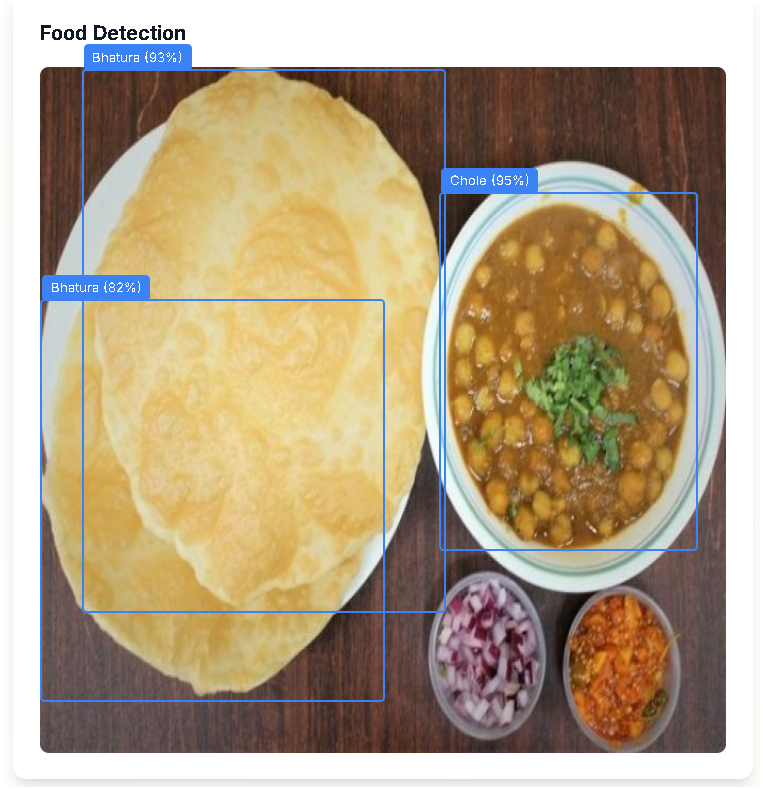
\includegraphics[width=0.88\linewidth,height=0.24\textheight,keepaspectratio]{detection_overlay.png}
\caption{Prototype output showing detected foods with bounding boxes and nutrition-linked results.}
\label{fig:prototype}
\end{figure}

The image-analysis response includes the detector label, display name, confidence, bounding box, image dimensions, macro values, nutrition source, and missing-nutrition flags. Runtime checks were run for classes that are easy to mishandle, including \code{aloo_gobi}, \code{palak_paneer}, \code{rice}, \code{AlooGobi}, and \code{WhiteRice}. These labels resolved to the expected nutrition rows. The API also returns an explicit no-food state when no valid detection is found.

\begin{table}[H]
\centering
\caption{Runtime behavior checked during prototype validation.}
\label{tab:runtime-validation}
\begin{tabular}{>{\raggedright\arraybackslash}p{0.34\linewidth}>{\raggedright\arraybackslash}p{0.49\linewidth}}
\toprule
Condition & Expected behavior\\
\midrule
\code{aloo_gobi} & Resolve to potato cauliflower nutrition row\\
\code{palak_paneer} & Resolve to spinach paneer nutrition row\\
\code{WhiteRice} & Normalize legacy label to boiled rice\\
No detected food & Return empty detections and no-food flag\\
Unmapped class & Preserve detection and mark nutrition unavailable\\
\bottomrule
\end{tabular}
\end{table}

\FloatBarrier

\section{Validation Scope}
\suppressfloats[t]

Validation was performed at several levels because the user-facing nutrition result depends on more than detector accuracy alone. Dataset checks confirmed class folders, label files, split counts, and visual samples. Model evaluation measured detection performance on validation and archived test splits. Nutrition checks verified that detector classes resolve to complete macro rows. Runtime checks confirmed that the backend response contains the fields required for overlays, nutrition display, serving controls, and recommendation prompts.

\begin{table}[H]
\centering
\caption{Validation layers used in the project.}
\label{tab:validation-layers}
\begin{tabular}{>{\raggedright\arraybackslash}p{0.30\linewidth}>{\raggedright\arraybackslash}p{0.52\linewidth}}
\toprule
Layer & What was checked\\
\midrule
Dataset & Split counts, class coverage, visual samples, annotation issues\\
Detector & Precision, recall, mAP@50, mAP@50:95, prediction examples\\
Nutrition & Database rows, mapping coverage, macro completeness, sources\\
API & Upload validation, no-food state, mapped and unmapped detections\\
Frontend & Overlay rendering, nutrition cards, serving controls, recommendations\\
\bottomrule
\end{tabular}
\end{table}

\FloatBarrier

The layered validation separates failure modes that would otherwise be hidden inside a single demonstration. A detector can classify a food correctly while the nutrition service maps it poorly. A nutrition database can contain complete rows while the frontend receives fields under unexpected names. Reporting these checks separately makes the system easier to audit and clarifies what has, and has not, been validated.

\section{Discussion}

The results show that nutrition-aware food recognition cannot be evaluated by detector mAP alone. A visually correct prediction can still produce an incorrect dietary result if it is mapped to the wrong food-composition row. The mapping table, source metadata, and explicit missing-value behavior are therefore part of the technical pipeline, not only backend implementation details.

The system also reflects a practical trade-off. It does not attempt exact portion estimation from a single image, because that would require assumptions that are difficult to verify in ordinary user photographs. Instead, it reports database-backed macro values and lets the user adjust gram-based portions. This limits automation, but it keeps the reported nutrition values closer to the evidence available to the system.

\section{Limitations}

The system does not estimate food mass, verify recipe ingredients or establish medical suitability. Detection performance has not been reassessed independently after the leakage findings. All mappings, including high-scoring entries, require independent evaluation; 21 have heuristic review flags. Source-family inference cannot rule out differently named crops or recompressed copies. Upstream augmented variants and annotation conflicts need review before a benchmark is frozen. Asset rights and author approval remain unresolved.

\section{Conclusion}

This work implements \textit{AI-Based Food Recognition with Nutrition-Aware Recommendations} as an educational web application and audits the evidence behind its detector and nutrition layer. The existing model and 72-class export remain unchanged. Exact cross-split duplication and unresolved source-family relationships prevent interpreting the archived detector metrics as independent generalization. The mapping layer provides lookup coverage for all 72 classes, but independent recipe-equivalence assessment is outstanding. Gram-based review, saved-only daily totals, explicit source details, and response-context labels improve inspectability; software tests do not establish clinical validity. The next research milestone is reviewed source grouping and annotation handling followed by a frozen evaluation protocol, appropriate retraining or untouched external testing, and independent mapping assessment. Asset permissions and author approval remain prerequisites for submission.

\FloatBarrier

\section*{Acknowledgment}

The implementation and dataset engineering artifacts used in this manuscript were developed as part of a final year project in the Department of Computer Science and Engineering, National Institute of Technology Srinagar. The authors acknowledge the technical supervision and review provided by project guide \guide\ and project co-guide \coguide.

\bibliographystyle{IEEEtran}
\bibliography{bibliography/references}

\end{document}
